% *** LaTeX-mal for labrapporter i fysikk, v.14.08.2017 ***

% Dette er et eksempel på et LaTeX-dokument, og du kan bruke dette som et utgangspunkt for din egen rapport. Merk at for å kunne kompilere dokumentet uten feil, må du også laste ned filen pendel-oppdatert.pdf.
%
% Her i starten og videre nedover i teksten under har vi lagt inn en god del linjer som starter med tegnet "%". Disse linjene er kommentarer og synes ikke i det ferdige dokumentet. Vi kan også sette inn et kommentartegn midt på en linje. Alt som kommer før tegnet brukes da i kompileringen, mens resten av linja er en kommentar.
%
% Kildefilen (.tex-filen) begynner alltid med et "preabmle". Her setter man opp innstillingene som brukes av kompilatoren til å utforme det ferdige dokumentet. Selve dokumentet begynner ikke før vi skriver \begin{document}.
%
% Dokumentasjon for alle pakker finnes på CTAN (http://www.ctan.org/)

%%%%%%%%%%%%%%%%%%%%%%%%%%%%%%%%%%%%%
% Preamble
%%%%%%%%%%%%%%%%%%%%%%%%%%%%%%%%%%%%%

\documentclass[5p,sort&compress]{elsarticle}
% 5p gir 2 kolonner pr side. 1p gir 1 kolonne pr side.
% Valget sort&compress gjør at referansen [1,2,3] settes som [1-3].
% Andre innstillinger for "klassen" elsarticle finnes i dokumentasjonen på CTAN (http://www.ctan.org/pkg/elsarticle)

% Klassen elsarticle er laget for bruk i engelskspråklige tiksskrift. I blokken under bruker vi litt lavnivå TeX-magi for å redefinere bunnteksten på tittelsiden. Ikke bekymre deg for denne biten med kode, det som kommer lengere nede i dokumentet er lettere å forstå!
\makeatletter
\def\ps@pprintTitle{%
 \let\@oddhead\@empty
 \let\@evenhead\@empty
 \def\@oddfoot{\footnotesize\itshape
      	% Bytt ut "Veileder" med navnet på veilederen din!
       \hfill\today}%
 \let\@evenfoot\@oddfoot}
\makeatother

% Encoding for input i tex-filen og encoding for output i pdf-filen
\usepackage[utf8]{inputenc}
\usepackage[T1]{fontenc}
\usepackage{textcomp}



% Last inn en font-pakke. Her bruker vi standard-fonten til LaTeX.
\usepackage{lmodern}

% LaTeX gjør mye av typografien for deg, blant annet orddeling ved linjeskift og automatisk utfylling av endel tekst. For å kunne gjøre dette må kompilatoren vite hvilket språk dokumentet er skrevet på.
\usepackage[english]{babel}
\usepackage[fixlanguage]{babelbib}
% Til tross for at vi har fortalt kompilatoren at vi skriver på engelsk må vi fortelle den eksplisitt at vi ønsker at seksjonen "abstract" skal kalles "sammendrag"
\renewenvironment{abstract}
{\global\setbox\absbox=\vbox\bgroup
\hsize=\textwidth\def\baselinestretch{1}%
\noindent\unskip\textbf{Summary}
\par\medskip\noindent\unskip\ignorespaces}
{\egroup}
% Mikrotypografiske optimeringer
\usepackage[babel=true]{microtype}


% AMS-utvidelsene for å håndtere matematikk
\usepackage{amsmath}
\usepackage{algpseudocode}
\usepackage{amssymb}
\usepackage{bm}
\usepackage{pifont}
\usepackage{tabularx}
\usepackage{multirow}
\usepackage{siunitx}
\usepackage{chngcntr}
\usepackage{tasks}
\usepackage{subcaption}
\usepackage{caption}
\usepackage{booktabs}
\newcommand{\ra}[1]{\renewcommand{\arraystretch}{#1}}
\usepackage{booktabs}
\usepackage{colortbl}
\usepackage{xcolor}
\usepackage{xfrac}
\usepackage{multicol}
\usepackage{float}
\usepackage[toc,page]{appendix}
\usepackage{listings}
\usepackage{comment}
% Måltall og enheter er spesielle typografiske dyr som reguleres av strenge regler. For å gjøre det enklere å håndtere tall og enheter på riktig måte bruker vi pakken siunitx.
\usepackage{siunitx}
% Vi tilpasser standardinstillingene til pakken til norske regler.
\sisetup{
exponent-product = \cdot,
output-decimal-marker  =  {,}, % Pass på å endre desimalskilletegnet til punktum om du skriver på engelsk!
separate-uncertainty = true,
per-mode = symbol,
group-digits = false,
}

% Figurer og tabeller
\usepackage{graphicx} % Denne pakken er standard for å kunne laste inn figurfiler med ulike formater
% Løsne opp på de alt for strenge standardinstillingene for plassering av figurer og tabeller (floats) i LaTeX-kjernen
\renewcommand{\topfraction}{.85}
\renewcommand{\bottomfraction}{.7}
\renewcommand{\textfraction}{.15}
\renewcommand{\floatpagefraction}{.66}
\setcounter{topnumber}{3}
\setcounter{bottomnumber}{2}
\setcounter{totalnumber}{10}
\usepackage{flafter} % For å plassere floats i PDFen første sted LaTeX tillater etter det punktet de er definert i TeX-filen. Om du definerer figuren i TeX-filen rett etter at du refererer til den for første gang vil denne pakken sørge for at de fleste floats havner på greie steder
\usepackage{booktabs} % Denne pakken gir tilgang på endel ekstra kommandoer som legger til rette for god skikk og bruk i tabellformatering.
\usepackage{multirow}
\usepackage[font=small,labelfont=bf]{caption}	% Justering av LaTeX standarder for figurtekst og tabelltekst.
\usepackage{algorithm2e}
\usepackage{algorithm}
\usepackage{amsmath}
\usepackage{algpseudocode}
\usepackage{varwidth}
\counterwithin{figure}{section}


\lstset{
frame = single,
language=Pascal,}

\definecolor{codegreen}{rgb}{0,0.6,0}
\definecolor{codegray}{rgb}{0.5,0.5,0.5}
\definecolor{codepurple}{rgb}{0.58,0,0.82}
\definecolor{backcolour}{rgb}{0.95,0.95,0.92}

\lstdefinestyle{mystyle}{
    backgroundcolor=\color{backcolour},
    commentstyle=\color{codegreen},
    keywordstyle=\color{magenta},
    numberstyle=\tiny\color{codegray},
    stringstyle=\color{codepurple},
    basicstyle=\ttfamily\footnotesize,
    breakatwhitespace=false,
    breaklines=true,
    captionpos=b,
    keepspaces=true,
    numbersep=5pt,
    showspaces=false,
    showstringspaces=false,
    showtabs=true,
    tabsize=2
}

\lstset{style=mystyle}

% Hyperreferanser
\usepackage[colorlinks=true,allcolors=blue]{hyperref}
% Noen av navnene for autoreferanser mangler på norsk, så vi ordner opp i det.
%\addto\extrasnorsk{%
%\def\figureautorefname{figur}%
%\def\tableautorefname{tabell}%
%\def\sectionautorefname{avsnitt}%
%\def\subsectionautorefname{underavsnitt}%
%}
% Vi endrer fonten som brukes for URLer til den vanlige tekstfonten.
\urlstyle{same}
% legge til pdf-er
\usepackage{pdfpages}


%%%%%%%%%%%%%%%%%%%%%%%%%%%%%%%%%%%%%
% Selve dokumentet
%%%%%%%%%%%%%%%%%%%%%%%%%%%%%%%%%%%%%

\begin{document}

% I "front matter" angir vi formalia knyttet til dokumentet -- tittel, forfatter, tilknytning og sammendrag
\begin{frontmatter}


\title{FYS-STK4155 - Project 1}
% I forfatterlisten legger vi inn "ikke-brytende" mellomrom etter initialene
\author[CS:PH]{A.~Isene}
\author[CS:IM]{C.D.~Nguyen}
\author[ROBOTIKK]{D.~Fremming}

\address[CS:PH]{UiO, Computational Science: Physics.}
\address[CS:IM]{UiO, Computational Science: Imaging and Biomedical Computing.}
\address[ROBOTIKK]{UiO, Robotics and Intelligent Systems.}

\begin{abstract}
    This is the summary
\end{abstract}

\end{frontmatter}

\newpage


\newpage
\section{Exercise 1: Expectation values for ordinary least squares expressions}
Assumptions:
\begin{enumerate}
    \item $\varepsilon \text{ is independent from } x \text{ which gives: }\mathbb{E}[\varepsilon]=0)$
    \item $y=f(x) + \varepsilon$ \text{. Here we will simplify f=f(x)}.
    \item $f(x) \text{ is a fixed, deterministic function of } x \text{, hence }\\ \mathbb{E}[f(x)]=f(x)$
\end{enumerate}
\hfill\break
\subsection{The mean-square error of our model can be written:}
%
%_____________________________________
%
\begin{align*}
    & \text{MSE} = \mathbb{E}[(y-\Tilde{y})^2]\\
    & = \mathbb{E}[y^2-2y\Tilde{y}+\Tilde{y}^2]\\
    & = \mathbb{E}[y^2]-2\mathbb{E}[y\Tilde{y}]+\mathbb{E}[\Tilde{y}^2]\\
\end{align*}
%
We look into each term:
\begin{equation}
\mathbb{E}[y^2]
\end{equation}
\begin{equation}
    \mathbb{E}[y\Tilde{y}]
\end{equation}
\begin{equation}
    \mathbb{E}[\Tilde{y}^2]
\end{equation}
%
%Term 1 ____________
From (1) we have:
 \begin{align*}
     & \mathbb{E}[y^2]=\mathbb{E}[(f+\varepsilon)^2]=\mathbb{E}[f^2+2f\varepsilon+\epsilon^2]\\
     & = \mathbb{E}[f^2]+\mathbb{E}[\varepsilon^2]\\
     & =  \mathbb{E}[f^2]+\sigma^2 = f^2+\sigma^2
 \end{align*}
%Term 2 _________________
From (2):
\begin{align*}
    & \mathbb{E}[y\Tilde{y}]=\mathbb{E}[y]\mathbb{E}[\Tilde{y}]
     = \mathbb{E}[f+\varepsilon]\mathbb{E}[\Tilde{y}]\\
    & =\mathbb{E}[f]\mathbb{E}[\Tilde{y}]=f\mathbb{E}[\Tilde{y}]
\end{align*}
%Term 3 _________________
We have:
\begin{align*}
    & Var[\Tilde{y}]=\mathbb{E}[(\Tilde{y}]-\mathbb{E}[\Tilde{y}])^2]\\
    & = \mathbb{E}[\Tilde{y}^2-2\Tilde{y}\mathbb{E}[\Tilde{y}]+(\mathbb{E}[\Tilde{y}])^2]\\
    & = \mathbb{E}[\Tilde{y}^2]-2\mathbb{E}[\Tilde{y}]\mathbb{E}[\Tilde{y}]+(\mathbb{E}[\Tilde{y}])^2\\
    & = \mathbb{E}[\Tilde{y}^2]-(\mathbb{E}[\Tilde{y}])^2\\
    & \implies \mathbb{E}[\Tilde{y}^2]= Var[\Tilde{y}]+(\mathbb{E}[\Tilde{y}])^2
\end{align*}
%
Put the terms together:
\begin{align*}
    & \mathbb{E}[y^2]-2\mathbb{E}[y\Tilde{y}]+\mathbb{E}[\Tilde{y}^2]\\
    & = f^2+\sigma^2-2f\mathbb{E}[\Tilde{y}]+(Var(\Tilde{y})+(\mathbb{E}[\Tilde{y}])^2)\\
    & = f^2-2f\mathbb{E}[\Tilde{y}]+(\mathbb{E}[\Tilde{y}])^2+Var(\Tilde{y})+\sigma^2\\
    & \implies \mathbb{E}[(f-\mathbb{E}[\Tilde{y}])^2]+Var(\Tilde{y})+\sigma^2
\end{align*}

First term in above expression can be approximated:
\begin{equation}
    \mathbb{E}[(f-\mathbb{E}[\Tilde{y}])^2] \simeq \frac{1}{n}\sum_{i}(y_i-\mathbb{E}[\Tilde{y}])^2 \text{ ,where } f_i\simeq y_i
\end{equation}

From (4) we have that MSE can be written:
\begin{equation}
    \mathbb{E}[(f-\mathbb{E}[\Tilde{y}])^2] \simeq \frac{1}{n}\sum_{i}(y_i-\mathbb{E}[\Tilde{y}])^2 = Bias[\Tilde{y}]
\end{equation}

Similarly, the variance can be expressed as:
\begin{align*}
    \mathbb{E}[(\Tilde{y}-\mathbb{E}[\Tilde{y}])^2]\simeq\frac{1}{n}\sum_{i}(\Tilde{y_i}-\mathbb{E}[\Tilde{y}])^2 = Var[\Tilde{y}]
\end{align*}
%___________________________________________
Setting in both the bias and variance terms into the equation we then obtain:

$MSE=Bias(\Tilde{y})+Var(\Tilde{y})+\sigma^2$

\subsection{Discussing the terms}
\hfill\break
The bias term represents the error caused by in-built assumptions in our used method. It consists of the average prediction over all data sets subtracted with the desired regression function.
The variance term describes the difference between solutions for the data sets and their average(variance of the model arounds its mean) \cite{bishop_2006_pattern}.

As for the sigma term, it represents the variance of the error, i.e. the noise of our method, where this quantity is expected to be irreducible. Since the sigma term is irreducible we will omit its interpretation in this section. The equation of minimum squared error(MSE) can be regarded as the expected loss when using our regression model, where we desire to minimize the error. This minimization can be dubbed the bias-variance trade-off, since it is about striking a balance between the bias and variance term. As for interpreting the terms(bias and variance), we will look into 2 scenarios as to how model complexity affects their behaviour.
Let $\Tilde{y}$ denote our model. The more complex it is, the better it is to go through the data points, hence we will acquire a lower bias. Respectively, the variance will be higher because the a higher model complexity makes the model "move" through more data points and it learns the noise of the training data. This flexibility in the model will lead run into the problem of overfitting our model, it works well on the training data we input, but it will run into problems once given new data it has never "seen", i.e. overfitting makes the model less able to generalize.

If the model $\title{y}$ is too rigid, it will output a high bias and low variance, and the model is not sufficient to fit the data points - we say it will underfit. Similarly to the case with a  complex model, it will result in a poor generalization.





\hfill\break
%
\section{Studying MSE values through analysis of Bias-variance}
%
% Set background color and other options for lstlisting

\hfill\break
The main code is obtained from: \url{https://compphysics.github.io/MachineLearning/doc/LectureNotes/_build/html/chapter3.html#the-bias-variance-tradeoff.}
\hfill\break
Modified code uses $y=sin(x)+log(x^2)$ as the one-dimensional function.


    \begin{lstlisting}[language=Python]
    import matplotlib.pyplot as plt
    import numpy as np
    from sklearn.linear_model import LinearRegression, Ridge, Lasso
    from sklearn.preprocessing import PolynomialFeatures
    from sklearn.model_selection import train_test_split
    from sklearn.pipeline import make_pipeline
    from sklearn.utils import resample

    np.random.seed(2018)

    n = 40
    n_boostraps = 100
    maxdegree = 14


    # Make data set.
    x = np.linspace(-3, 3, n).reshape(-1, 1)
    y = np.sin(x) + np.random.normal(0, 0.1, x.shape)
    error = np.zeros(maxdegree)
    bias = np.zeros(maxdegree)
    variance = np.zeros(maxdegree)
    polydegree = np.zeros(maxdegree)
    x_train, x_test, y_train, y_test = train_test_split(x, y, test_size=0.2)

    for degree in range(maxdegree):
        model = make_pipeline(
            PolynomialFeatures(degree=degree), LinearRegression(fit_intercept=False)
        )
        y_pred = np.empty((y_test.shape[0], n_boostraps))
        for i in range(n_boostraps):
            x_, y_ = resample(x_train, y_train)
            y_pred[:, i] = model.fit(x_, y_).predict(x_test).ravel()

        polydegree[degree] = degree
        error[degree] = np.mean(np.mean((y_test - y_pred) ** 2, axis=1, keepdims=True))
        bias[degree] = np.mean((y_test - np.mean(y_pred, axis=1, keepdims=True)) ** 2)
        variance[degree] = np.mean(np.var(y_pred, axis=1, keepdims=True))
        print("Polynomial degree:", degree)
        print("Error:", error[degree])
        print("Bias^2:", bias[degree])
        print("Var:", variance[degree])
        print(
            "{} >= {} + {} = {}".format(
                error[degree],
                bias[degree],
                variance[degree],
                bias[degree] + variance[degree],
            )
        )

    plt.plot(polydegree, error, label="Error")
    plt.plot(polydegree, bias, label="bias")
    plt.plot(polydegree, variance, label="Variance")
    plt.legend()
    plt.show()
    \end{lstlisting}
Results from the bias and variance trade-off as function of the model complexity can be seen in the table ~\ref{tab:ModelComplexMSE} below.
Here we set the number of data points to 40 and bootstrap to 100 iterations.
Blue rows highlights where the model complexity yields the lowest error:

\begin{table}
    \centering
    \begin{tabular}{c|c|c|c}
        \textbf{Order} & \textbf{Error} & \textbf{Bias\textsuperscript{2}} & \textbf{Variance}\\
        \text{0} & 3.222694  & 3.104592   & 0.118102\\
        \text{1} & 2.637989  & 2.492254   & 0.145734 \\
        \text{2} & 1.234957 & 1.095855    & 0.139102\\
        \text{3} & 1.142538 & 0.978143   & 0.164395\\
        \text{4} & 0.604439 & 0.475311  & 0.129127\\
        \text{5} & \cellcolor{blue!25}0.578585 & \cellcolor{blue!25}0.4131747   & \cellcolor{blue!25}0.165410\\
        \text{6} & \cellcolor{blue!25}0.370845 & \cellcolor{blue!25}0.214435   &  \cellcolor{blue!25}0.156410\\
        \text{7} & \cellcolor{blue!25}0.435129 & \cellcolor{blue!25}0.229928  & \cellcolor{blue!25}0.205200\\
        \text{8} & 0.739773 & 0.360638   & 0.379134\\
        \text{9} & 1.179098 & 0.368951   & 0.810147 \\
        \text{10} & 0.917037& 0.390615   & 0.526421 \\
        \text{11} & 7.420075 & 0.278572  & 7.141503  \\
        \text{12} & 9.530186 & 0.267499  & 9.262687  \\
        \text{13} & 16.252874 & 0.147212 & 16.105661 \\
    \end{tabular}
    \caption{Bias and variance trade-off as function of polynomial complexity.}
    \label{tab:ModelComplexMSE}
\end{table}

\begin{figure}
    \centering
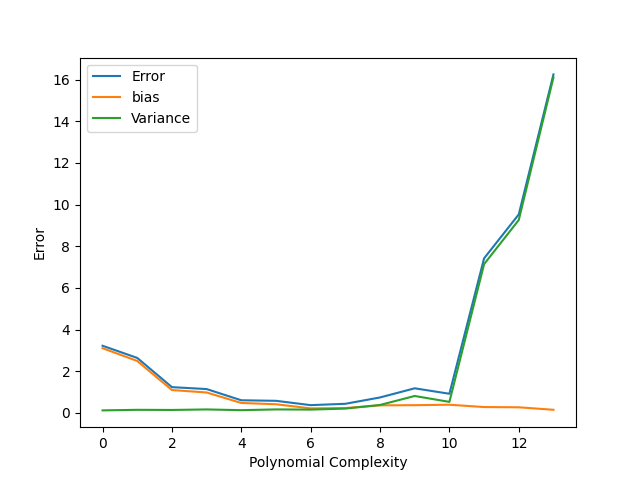
\includegraphics[width=1.0\linewidth]{figures/Figure_1.png}
    \caption{Plot Analysis of  plot of error, bias, and variance as function of increasing complexity}
    \label{fig:1}
\end{figure}

\newpage
\section{Bias-Variance Trade-Off}
%
\begin{itemize}
    \item \textbf{Low Complexity($<5$):} High bias and low error, the model underfits our test data and is not able to capture the complexity of our target function. This gives us a somewhat higher error.
    \item \textbf{Optimal Complexity($5-7$):} Our error is relatively low meaning that our model does a decent job in describing underlying patterns in the target function. This is provided by the bias-term. The variance on the other hand, is low enough so our model does not overfit. For the polynomial degree between 4-7 we can see that the trade-off between bias and variance is minimizes the error.
    \item \textbf{High Complexity($>7$):} The low bias describes now that our model is exceptional at fitting to our target function, but our model is now too specific - it is restricted to perform well with the data set we provided, but will struggle with new data sets. The high variance shows that our model has been overfitted and the higher error describes that our model is no longer suitable for generalization.
\end{itemize}
%
From the table we can see the error of the model is at its lowest when the degree of the polynomial is 6. This also holds true for visual inspection of the graph in figure ~\ref{fig:1}.

\section{Effect of Number of Data Points}

\hfill\break
From quick plots we observed that for low function complexity, the error, bias and variance stayed low (closer to $0$, seemingly). A major difference is the magnitude of error. On the y-axis we observed the error for (data points = 10) to take values between 0-700. When setting number of data points to 70, the error decreased and was within the range 0-3.5, but the error, bias and variance stayed at an all time low of zero until a polynomial degree of 10.

\section{Bootstrap Resampling}
As for bootstrap resampling we worked with the following number of bootstraps while holding number of samples fixed: (10,200).
For number of bootstraps= 10 the error varied where the bias was approximate close to the error to begin with. The graph of bias and errors stayed the same until degree 11 where error and variance were dominant and closer to each other and suddenly made a jump(see~\ref{fig:2}).
As for number bootstrap= 200, we had another behaviour. As depicted in figure~\ref{fig:3}.

\begin{figure}
    \centering
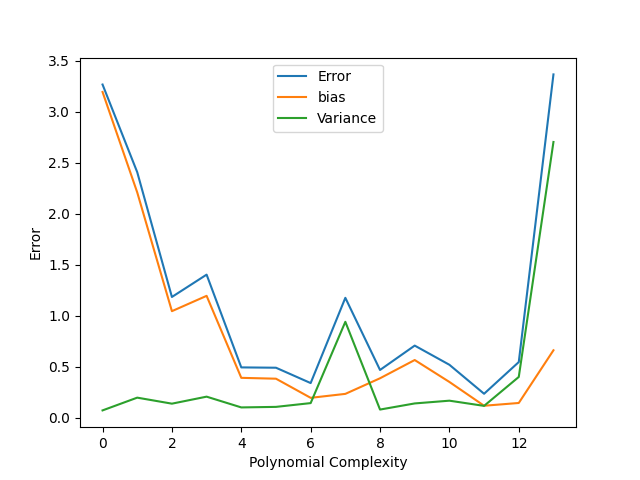
\includegraphics[width=1.0\linewidth]{figures/bootstrap 1.png}
    \caption{Plot Analysis of  plot of error, bias, and variance as function of increasing complexity}
    \label{fig:2}
\end{figure}

\begin{figure}
    \centering
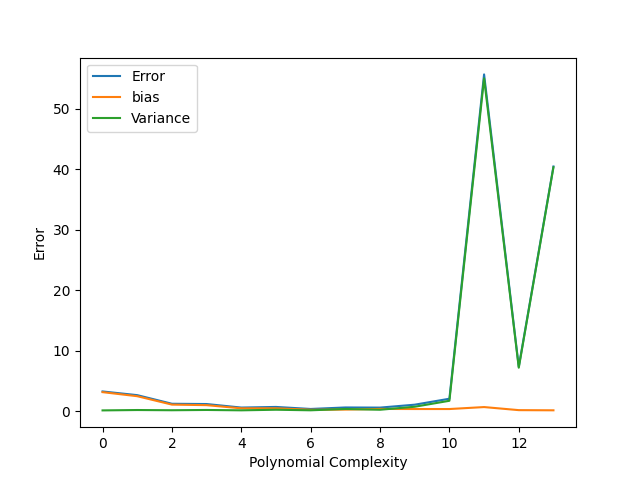
\includegraphics[width=1.0\linewidth]{figures/bootrstrap2.png}
    \caption{Plot Analysis of  plot of error, bias, and variance as function of increasing complexity}
    \label{fig:3}
\end{figure}




\end{document}
